\chapter{Securing Unmodified Applications}
\label{unmodified_app}
TEEs have been around for a long time now, and have been used for a diverse
range of applications as can be seen in section \ref{sec:related}. While these
bodies of research might target different problems, the way in which these projects
structure their secure applications roughly falls into three distinct categories which
differ based on the information being protected and the threat model around
which the application has been designed: 

%%%%%%%%%%%%%%%%%%%%%%%%%%%%%%%%%%%%%%%%%%%%%%%%%%%%%%%%
\begin{figure}[t]
    \centering
    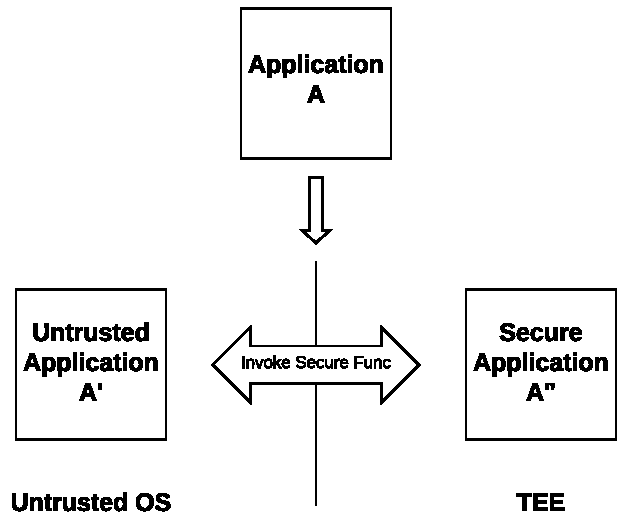
\includegraphics{fig/split_app.pdf}
    \caption{An application can be split into two parts - one that resides in the unstrusted operating system and has the interfaces to secure functionality that resides in the trusted environment.}
    \label{fig:split_app}
\end{figure}
%%%%%%%%%%%%%%%%%%%%%%%%%%%%%%%%%%%%%%%%%%%%%%%%%%%%%%%%



\begin{enumerate}
    \item \textbf{Manually Split the Application into Trusted and Untrusted
    Parts:} This is the most commonly used methodology designing applications
    with the view to use a TEE to safeguard some aspect of the program state 
    \cite{TLR,Proxos,SchrodinText,liu2014veriui}. 
    
    The basic idea is that there is some easily identifiable functionality that
    can be plucked out of the monolithic application and can be offloaded to the
    TEE. The rest of the application that remains on the untrusted OS only has
    interfaces to the secure functions in the TEE. This is shown in Figure
    \ref{fig:split_app}. The TEE in this scenario could either be a trusted
    operating sytem that is hosted as a virtual machine or it could be a
    more conventional hardware based TEE like Intel's SGX or ARM's TrustZone. 

    This application splitting paradigm is promising in scenarios where the
    critical functionality that needs protection is small, well defined, and can
    be extracted away into a TEE-resident service. Prime examples of this is
    biometric verification, cryptographic functions, payment processing, and
    verifying the user's action and intent. An implicit assumption with this
    strategy is that the partitioning of the application is a deliberate
    decision that is made at the time of designing the application, and
    therefore can not be used for unmodified application. 
    
    \item \textbf{Compiler Automatically Sequester the Applcation}: There has
    been work in securing application using comiler wizardry. VirtualGhost
    \cite{criswell2014virtual} defines a compiler based instrumentation of the
    kernel and the application to protect the applications data condifentiality
    and integrity. The OS is compiled to a virtual instruction set which is
    handled by the Virtual Ghost VM as shown in Figure \ref{fig:compiler_split}.
    This \say{virtual machine} is used to limit the accesses the kernel has into
    the state of the application. This is interesting work that provides strong
    guarantees about the application's integrity and data confidentiality
    without using a hardware based TEE. 
    
    There has been work in automatically identifying which parts of the
    application need to be protected and actually splitting the application
    using the TEE API \cite{rubinov2016automated, lind2017glamdring}. This
    approach involves using static analysis and dataflow analysis along with
    optoinal annotations in the program to automatically identify partitioning
    scheme, and then refactoring the application into two parts that are bridged
    using the TEE API. Programming language theory can be used to
    demonstate equivalence between the split halves and the original
    application. 

    These approaches might be an efficient way to retoactively make an
    unmodified application ready for a TEE.
    %%%%%%%%%%%%%%%%%%%%%%%%%%%%%%%%%%%%%%%%%%%%%%%%%%%%%%%%
    \begin{figure}[t]
        \centering
        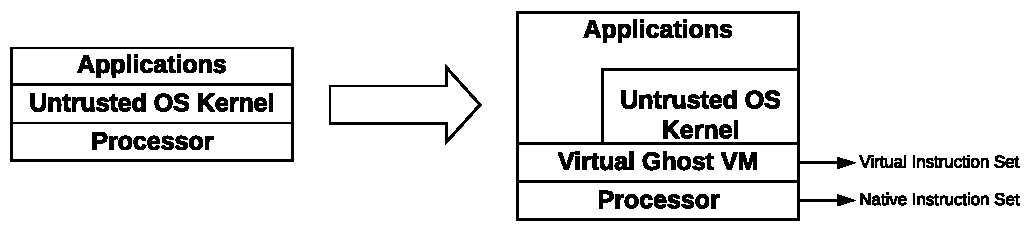
\includegraphics[width=\linewidth]{fig/compiler_split.pdf}
        \caption{Virtual Ghost uses LLVM to create an intermediate layer  the OS and the processor to protect the application from teh unfettered access otherwise enjoyed  by a kernel}
        \label{fig:compiler_split}
    \end{figure}
    %%%%%%%%%%%%%%%%%%%%%%%%%%%%%%%%%%%%%%%%%%%%%%%%%%%%%%%%

    \item \textbf{Complete Isolation of the Application Inside the Secure World}
    
    \item \textbf{System Call Interception }
    If the complete isolation of an application is not possible, and it is
    necessary to maintain some part of the application in the untrusted OS, the
    most enticing option available to the security engineer is to use system
    call interception in the normal world OS and handle the \say{sensitive}
    accesses to data and the network in the TEE. This approach can go awry if
    there is not a strict control on the number and type of system calls that
    are handled in the TEE - the more elaborate the handler in the TEE, the
    higher will be the slowdown, and less usable will be the system. 

    This approach can be used in some cases, however. In Hypervision
    \cite{hypervision}, the normal world kernels memory mangement is handled
    entirely from within TrustZone, thereby allowing opportunities for real-time
    monitoring of the normal world kernel. There is marginal performance
    deterioration in this case because there is very little code being executed
    in the TEE; the penalty arises from the cost to switch between the normal
    and the secure world. On the other hand, TrustedCapsule's first prototype
    was overtly ambitious in the amount of work that was being done on every
    single system call to a capsule file, causing in some cases a 300x slowdown
    on simple tasks such as opening a capsule. 
\end{enumerate}


All the systems presented in the related works section tend to focus on
applications that rely on a rather narrow set of services from the TEE.
Cryptography, SecureUI.